\documentclass[12pt,a4paper]{report}
\usepackage[brazil]{babel}
\usepackage[]{algorithm}
\usepackage[]{algorithmic}

\usepackage[style=numeric,backend=biber]{biblatex}
\usepackage[utf8]{inputenc}
\usepackage{kpfonts}
\usepackage[T1]{fontenc}
\usepackage{wrapfig}
\usepackage{graphicx}
\usepackage{enumerate}
\usepackage{subcaption}
\usepackage{float}
\usepackage{caption}
\usepackage{listings}
\usepackage{lipsum}
\usepackage{amsthm}
\usepackage{amssymb}
\usepackage{bm}
\usepackage{color}
\usepackage{afterpage}
\usepackage[inline]{enumitem}
\usepackage{pdflscape}
\usepackage{listingsutf8}
\usepackage{siunitx}
\usepackage{bashful}

\usepackage[margin=1in]{geometry}

\lstset{frame=tb,
  aboveskip=2mm,
  belowskip=2mm,
  showstringspaces=false,
  columns=flexible,
  basicstyle=\footnotesize,,
  numbers=left,
  numbersep=5pt,
  stepnumber=1,
  breaklines=true,
  keepspaces=true,
  breakatwhitespace=true,
  showtabs=false,  
  tabsize=2
}


% Definindo estilo para os códigos
\definecolor{mGreen}{rgb}{0,0.6,0}
\definecolor{mGray}{rgb}{0.5,0.5,0.5}
\definecolor{mPurple}{rgb}{0.58,0,0.82}
\definecolor{dkgreen}{rgb}{0,0.6,0}
\definecolor{backgroundColour}{rgb}{0.97,0.97,0.97}

\lstset{basicstyle=\ttfamily,
    backgroundcolor=\color{backgroundColour},   
    commentstyle=\color{mGreen},
    keywordstyle=\color{magenta},
    numberstyle=\tiny\color{mGray},
    commentstyle=\color{dkgreen},
    stringstyle=\color{mPurple},
    basicstyle=\footnotesize,
    breakatwhitespace=false\textbf{,}         
    breaklines=true,                 
    captionpos=b,                    
    keepspaces=true,                 
    numbers=left,                    
    numbersep=5pt,                  
    showspaces=false,                
    showstringspaces=false,
    showtabs=false,                  
    tabsize=2,
    language=bash
}

\lstdefinestyle{BStyle}{
    backgroundcolor=\color{backgroundColour},  
    showstringspaces=false,
    numbers=none,
    language=bash
}

\pagenumbering{arabic}
\renewcommand{\thesection}{\arabic{section}}

\bibliography{ref}
\renewcommand{\contentsname}{Sumário}{\thispagestyle{empty}}
\renewcommand{\baselinestretch}{1.5} 

\begin{document}

\begin{titlepage}
        \begin{center}
                \vspace*{1cm}
                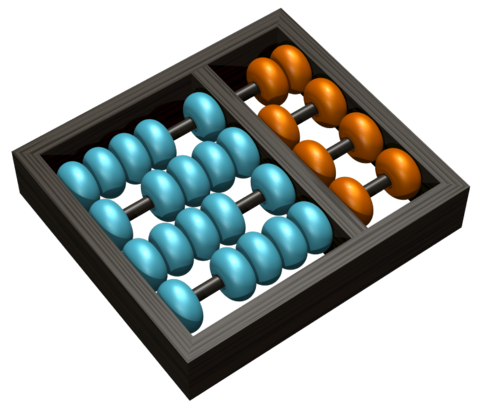
\includegraphics[width=0.25\textwidth]{Logo}\\
                \vspace{1.5cm}
                \Huge
                \textbf{Exercício 2}\\
                \vspace{1.5cm}
                \Large
                \textbf{Aluno}: João Vitor Gonçalves\\
                \textbf{RA}: 176353\\
                \vspace{1.2cm}
                \Large
                Instituto de Computação\\
                Universidade Estadual de Campinas\\
                \vspace{1.5cm}
                Campinas, 18 de Outubro de 2020.
        \end{center}
\end{titlepage}
\tableofcontents
\clearpage

\newcommand{\shellcmd}[1]{\texttt{\footnotesize\# #1}}%estilizando citação de comandos do shell

% \section{Insertion Sort}

% \subsubsection{Pseudocódigo}
% \begin{algorithm}
% \caption{InsertionSort(A)}
% \begin{algorithmic}[1]
%     \STATE $A[0] \longleftarrow -\alpha$
%   \STATE $i \longleftarrow 2 $
%     \FOR {$i$ to $N $} 
%             \STATE $j \longleftarrow i$

%             \WHILE{$A[j] > A[j-1]$} 
%                 \STATE $T \longleftarrow A[j-1]$ 
%                 \STATE $A[j-1] \longleftarrow A[j]$ 
%                 \STATE $A[j] \longleftarrow T$ 
%                 \STATE $j = j -1$
%             \ENDWHILE
%     \ENDFOR
%     \RETURN $A$
%     \end{algorithmic}
% \end{algorithm}



\section{Analise os códigos dos programas cliente.c e servidor.c e identifique as funções usadas para
comunicação via socket. Procure nas páginas de manual do Linux, a descrição das funções que
estão relacionadas ao uso de sockets. Procure também nos códigos a natureza dos parâmetros
que cada programa deve receber, se for o caso.}

Funções utilizadas para a comunicação via socket:

\begin{itemize}
  \item \textbf{socket(AF\_INET, SOCK\_STREAM, 0)}: 
  
  Trata-se do método:

  \emph{ int socket(int domain, int type, int protocol);}

  Que é utilizado para criar uma ponta de comunicação e retorna um \emph{file descriptor} que é utilizado para receber as transmissões desse socket.

  \bigbreak

  Onde o \emph{domain} determina o domínio de comunicação, que no caso de \textbf{AF\_INET}, identifica que será utilizado o protocolo IPv4.
  
  \bigbreak

  Já o \emph{type} identifica o tipo de comunicação usada, que no caso do \textbf{SOCK\_STREAM} 
  fornece uma comunicação confiável \emph{two-way} baseada em conexão(\emph{TCP}).

  \bigbreak

  Com o último parâmetro \emph{protocol}, é possível específicar que protocolo será utilizado, mas para a maioria dos tipos de socket, apenas um protocolo é suportado, e nesses casos é passado o valor \textbf{0}.

  \item \textbf{connect(sockfd, (struct sockaddr *) \&servaddr, sizeof(servaddr)}: 
  
  Trata-se do método:

  \emph{int connect(int sockfd, const struct sockaddr *addr, socklen\_t addrlen);}

  Que realiza a conexão ao socket referenciado pelo \emph{file descriptor} \textbf{sockfd} no endereço \textbf{addr}.

  O método retorna \emph{0} no caso de sucesso, e \emph{-1} no caso de erro.

  \item \textbf{bind(listenfd, (struct sockaddr *)\&servaddr, sizeof(servaddr))}: 

  Trata-se do método:

  \emph{int bind(int sockfd, const struct sockaddr *addr, socklen\_t addrlen);}

  Que é responsável por atribuir o endereço passado \textbf{addr} ao socket referenciado pelo \emph{file descriptor} \textbf{sockfd}. Uma vez que quando um socket é criado, ele não possui um endereço ainda, ele é criado apenas com uma família de endereços que ele pode ser atribuído.

  \item \textbf{listen(listenfd, LISTENQ)}
  
  Trata-se do método:

  \emph{int listen(int sockfd, int backlog);}

  Que é usado para marcar o socket passado como um socket passivo, que será utilizado apenas para aceitar conexões externas pelo método \emph{accept}.

  \bigbreak

  Os atributos passados são o \textbf{sockfd}, que é o \emph{file descriptor} do socket referenciado e o \textbf{backlog}, que determina o tamanho máximo da fila de conexões pendentes a serem conectadas.

  No caso do código do servidor, a constante \textbf{LISTENQ} está definida como 10.

  \item \textbf{int accept(listenfd, (struct sockaddr *) NULL, NULL)}

  Trata-se do método:

  \emph{int accept(int sockfd, struct sockaddr *addr, socklen\_t *addrlen);}

  Esse método é usado para aceitar uma conexão na fila de conexões pendentes para o socket referenciado pelo \emph{file descriptor} passado.

  Ele extrai a primeira conexão pendente na fila, cria um novo socket referenciando essa conexão, e retorna o seu \emph{file descriptor} para realização de conexões.

  \bigbreak

  Os parâmetros \textbf{sockaddr} e \textbf{addrlen} são preenchidos com os valores do socket criado, e no caso de eles não serem utilizado, pode ser passado o valor \emph{NULL} para o seus ponteiros, e esse preenchimento não será feito.

\end{itemize}

\bigbreak

Em relação aos parâmetros esperados pelos programas, o cliente.c espera que o endereço IP do servidor seja passado via argumento do programa. Já o servidor não espera nenhum argumento.

\section{Compile e execute os programas cliente.c e servidor.c em uma mesma máquina. Houve algum
erro? Em caso afirmativo, qual a sua causa? Se necessário, modifique os programas de forma
que este erro seja corrigido e informe quais modificações foram realizadas. (Insira uma figura
mostrando que o seu código executou sem erros)}

O código do cliente.c foi compilado com sucesso sem erros, já o código do servidor.c exibiu os seguintes \emph{warnings}:

\begin{lstlisting}[language=bash]
  gcc -o servidor servidor.c

  servidor.c: In function `main':
  servidor.c:33:37: warning: passing argument 1 of `htonl' makes integer from pointer without a cast [-Wint-conversion]
     33 |    servaddr.sin_addr.s_addr = htonl("192.168.0.16");
        |                                     ^~~~~~~~~~~~~~
        |                                     |
        |                                     char *
  In file included from /usr/include/netdb.h:27,
                   from servidor.c:5:
  /usr/include/netinet/in.h:378:33: note: expected `uint32_t' {aka `unsigned int'} but argument is of type `char *'
    378 | extern uint32_t htonl (uint32_t __hostlong)
        |                        ~~~~~~~~~^~~~~~~~~~
\end{lstlisting}

Causado pela linha: \emph{servaddr.sin\_addr.s\_addr = htonl(``192.168.0.16'');}

Isso é pelo fato de que o método \emph{htonl} aceitar um valor do tipo `uint32\_t' como parâmetro, e não \emph{char *}, como é o caso. 

\bigbreak

Para isso, essa linha foi substituida pelo método: 

\emph{inet\_pton(AF\_INET, ``192.168.0.16'', \&(servaddr.sin\_addr));}

Que segundo o manual do linux, converte um endereço passado em forma de string para um \emph{network address}, e o preenche no destino passado, que no caso é: \textbf{\&(servaddr.sin\_addr)}.

E o primeiro parâmetro determina que tipo de endereço será passado, que no caso do IPv4 é \textbf{AF\_INET}.


\bigbreak

Agora o servidor.c compila sem erros, porém ao executa-lo, é retornado o seguinte erro: \emph{bind: Cannot assign requested address}.

Isso ocorre devido ao endereço IP passado \emph{192.168.0.16} não é o IP local na rede da interface de rede utilizada. Para corrigir esse problema, o endereço foi trocado pelo endereço ``localhost'', ou \emph{127.0.0.1}.

\bigbreak

Porém agora o servidor exibe o erro \emph{bind: Permission denied}, e só executa com sucesso executando o processo com \emph{sudo}. Isso ocorre devido à porta utilizada: \emph{13}. Uma vez que portas inferiores à \emph{1024} são consideradas privilegiadas.

Para não precisar executar o processo em modo administrador, a porta usada foi simplesmente trocada para \emph{8585}.

\bigbreak

Então naturalmente após também trocar a porta utilizada no cliente para \emph{8585}, ambos os programas executam com sucesso.

\begin{figure}[H]
  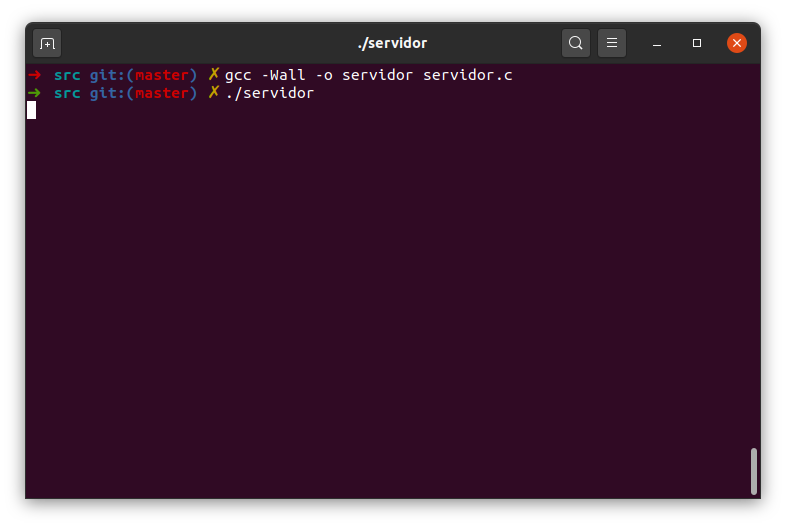
\includegraphics[width=\linewidth]{servidor.png}
  \caption{Compilação e execução do servidor com sucesso.}
\end{figure}

\begin{figure}[H]
  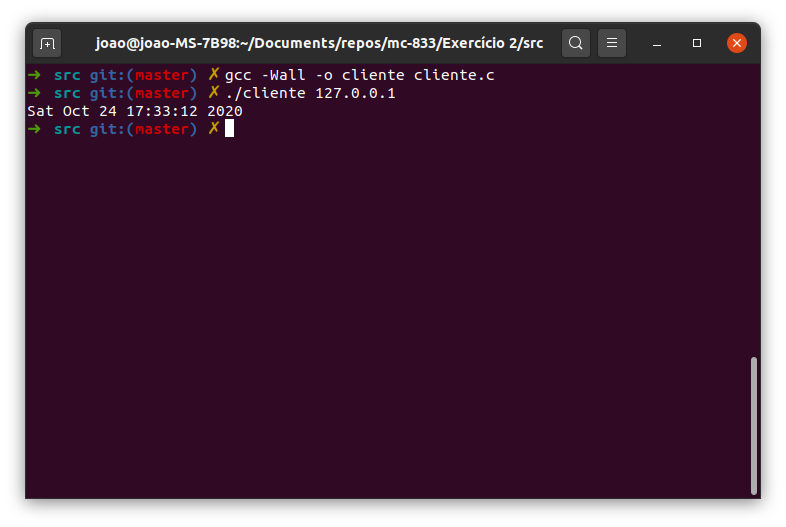
\includegraphics[width=\linewidth]{cliente.png}
  \caption{Compilação e execução do cliente com sucesso.}
\end{figure}

\section{Altere o código do servidor para que seja automatizado a escolha da porta e utilize sempre o
IP da máquina que está sendo executado.}


\section{Liste as chamadas de sistema necessárias para um servidor escutar conexões futuras.
Justifique.}

\section{Adicione comentários necessários ao código. (Não precisa anexar esta questão no relatório. Os
comentários serão analisados no código enviado)}

\section{Modifique o programa cliente.c para que ele obtenha as informações do socket local (\# IP, \#
porta local) através da função getsockname().}

\section{Modifique o programa servidor.c para que este obtenha as informações do socket remoto do
cliente (\# IP remoto, \# porta remota), utilizando a função getpeername(). Imprima esses
valores na saída padrão.}

\section{É possível usar o programa telnet no lugar do binário do cliente.c? Justifique e comprove sua
resposta.}

\end{document}